\section{Implementation}

\subsection{System Architecture}

The architecture of the system we proposed can be seen in
figure \ref{system-architecture}.
We can separate the deployment into 4 groups.
\begin{enumerate}
    \item The first one, the ESP32, are the physical device
          that gathers the air quality data and controls the door.
    \item Second, the Application Server are the primary brain
          of the whole system from collecting the data
          retrieved from the ESP32, saving the data, to
          managing the state of the system.
    \item Third, the SparkMachine, are the processor of data
          that processes the data into more meaningful
          informations for the user, such as minimum, maximum,
          and average values.
    \item Lastly, the User Device are users' devices that
          accesses the web application to interact with the
          system.
\end{enumerate}

\begin{figure*}
    \centering
    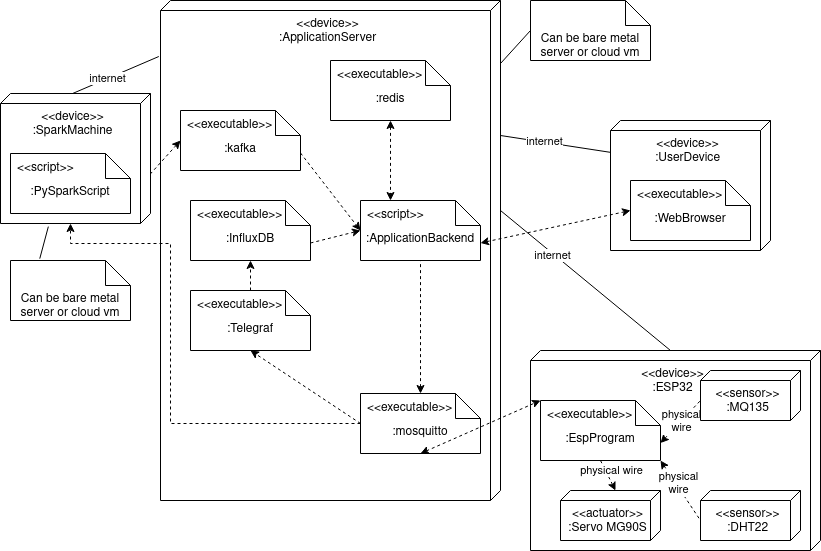
\includegraphics[scale=0.5]{resources/deployment-diagram.png}
    \caption{Deployment diagram of the smart room air conditioner}
    \label{system-architecture}
\end{figure*}

Flow-wise, the data gathered by the MQ135 and DHT22, in the
ESP32, are sent to the mosquitto, the MQTT broker, in the
Application Server.
There, the data are consumed by both Telegraf in the
Application Server to be saved into the InfluxDB, and
PySparkScript in the SparkMachine to be processed into
minimum, maximum, average, and median values.

The sensor data in InfluxDB and the processed data are then
used to be displayed as a statistic of the web application.
The sensor data are also used as training data for the KMeans
algorithm to determine the air quality level of each
indicators. The current average of each indicators are then
passed to the KMeans model to determine the current air
quality level of the room, thus determining whether the door
should be opened or closed.

\subsection{Machine Learning Model}
Since the data gathered by the sensors are time
series data, we will use Time Series KMeans (TSKM)
algorithm to cluster the data, that is provided in
python by
\href{https://tslearn.readthedocs.io/en/stable/}{\texttt{tslearn}} library.
KMeans algorithm are chosen because it is simple and
easy to implement, and it is also one of the most
popular clustering technique.

To train the model, we used the data gathered by the
sensors for 3 days, as the InfluxDB database stores,
from 2021-05-01 to 2021-05-03. Since the data,
especially from the MQ135 sensor were not too
accurate, we ``smoothened'' the data by using the
\href{https://pandas.pydata.org/docs/reference/api/pandas.DataFrame.rolling.html}{\texttt{rolling}} mean, which saves
the mean of the current rolling window of 120 data. The number
120 is chosen arbitarily to ensure the data is smooth enough,
but not too smooth that it loses its meaning. We also used 2
clusters for the model, as we only need to separate the data
into ``good'' and ``bad'' air quality.

The result of the training can be seen in
figure \ref{kmeans}. Due to use of clustering algorithm, we could not
determine the exact value of each indicators that is the
discriminant point that separates the ``good'' and ``bad''
air quality, but we can see that the ``good'' air quality is
represented by the lower part, and the ``bad'' air quality is
represented by the upper part.

We then implement the model into the system by passing each
indicators' current average value to the model to determine
the current air quality level of the room. The result of the
model is then used to determine whether the door should be
opened or closed using the following rules:
\begin{enumerate}
    \item If the CO2 level is ``bad'', the door will not be
          opened, since we don't want any toxic particles to
          get in the room.
    \item If the CO2 level is ``good'', we will check the
          next indicators, temperature and humidity. If
          either temperature or humidity is ``bad'', then the
          door will be opened, since we want to get fresh
          air into the room.
    \item If both temperature and humidity are ``good'',
          then the door will not be opened, since the air
          quality is already good.
\end{enumerate}


\begin{figure}
    \centerline{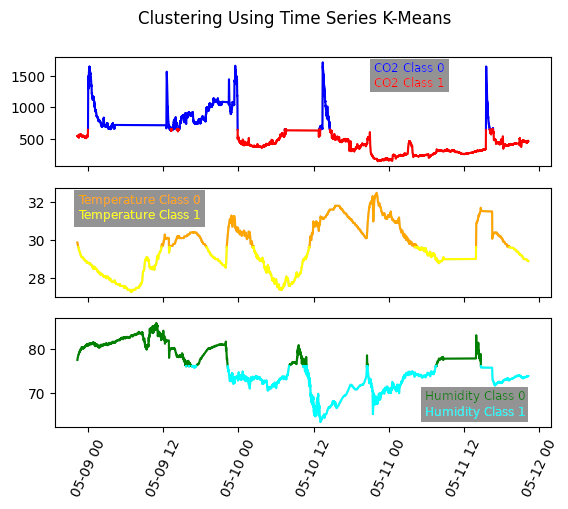
\includegraphics[scale=0.65]{resources/iot-clustering.png}}
    \caption{Time Series KMeans clustering result visualization}
    \label{kmeans}
\end{figure}